\chapter{Funktionen}

Bislang sahen alle deine Programme folgendermaßen aus:

\begin{minipage}{\textwidth}
\begin{lstlisting}
public class Funktionen {
  public static void main(String[] args) {
    //do something
  }
}
\end{lstlisting}
\end{minipage}

Auch hier hast du schon eine Funktion verwendet, möglicherweise ohne es zu wissen: \textit{public static void main(String[] args)} definiert eine Funktion. Diese spezielle Funktion ist eine besondere: Sie deklariert für den Rechner den Einstiegspunkt in unser geschriebenes Programm. Euer Code wird beginnend in dieser Funktion ausgeführt. Ihr habt auch die Möglichkeit weitere Funktionen zu schreiben. Der Syntax dafür ist der folgende:

\begin{minipage}{\textwidth}
\begin{lstlisting}
public class Funktionen {
  public static void myFunction() {
    //do something
  }
}
\end{lstlisting}
\end{minipage}

Das erste Wort, \textit{public} ist ein Schlüsselwort, welches angibt wer diese Funktion benutzen kann. Ich möchte an dieser Stelle nicht in die Tiefe gehen, aber euch die möglichen Schlüsselwörter nicht vorenthalten:

\begin{itemize}
	\item \textit{public}
	\item \textit{private}
	\item \textit{protected}
\end{itemize}

Das zweite Schlüsselwort, \textit{static} sei für den Moment verpflichtend. Wenn ihr euch mit Objektorientierung beschäftigt, kann dieses Schlüsselwort ausgelassen werden. Das liegt aber außerhalb des Rahmen dieses Vorkurses.

Das dritte Schlüsselwort, \textit{void}, bezeichnet den Rückgabetyp einer Funktion. \textit{void} bedeutet dabei, dass diese Funktion keinen Rückgabetyp hat. Jede beliebige Bezeichnung eines Datentyps, zum Beispiel \textit{int, bool, String, ...} kann an dieser Stelle stehen. Wenn dort ein Datentyp stehen, muss diese Funktion einen Wert dieses Datentyps zurückgeben:

\begin{minipage}{\textwidth}
\begin{lstlisting}
public class Funktionen {
  public static int myFunction() {
    int someInt = 0;
    //do something
    return someInt;
  }
}
\end{lstlisting}
\end{minipage}

Das Schlüsselwort für das Zurückgeben eines Wertes ist \textit{return}. Wenn die Funktion \textit{return} erreicht hat, wird kein weiterer Code in der Funktion ausgeführt sondern sofort zurück in aufrufende Funktion gesprungen. In diesem Sinne funktioniert \textit{return} wie ein \textit{break}.

Diese Funktionen können nun genauso mit Code befüllt werden wie ihr bisher die \textit{main}-Funktion getan habt. Ein Beispiel ist das Folgende:

\begin{minipage}{\textwidth}
\begin{lstlisting}
public class Funktionen{
  //hier startet das Programm
  public static void main(String[] args){
    int number = readNumberFromConsole();
    bool isPrime = checkPrime(number);
    print(number, isPrime);
  }      
  
  public static int readNumberFromConsole(){
    int number;
    //you already should know the code for this
    return number;
  }
  
  public static bool checkPrime(int number){
    bool result;
    //you shall figure out this code for yourself
    return result;
  }
  
  public static void print(int number, bool isPrime){
    if(isPrime)
      System.out.println(number + " ist eine Primzahl");
    else
      System.out.println(number + " ist keine Primzahl");
  }
}
\end{lstlisting}
\end{minipage}

Das obenstehende Beispiel demonstriert die Verwendung von Funktionen. Manche Funktionen können Parameter besitzen, also Werte von denen diese Funktion abhängt. Bei der Definition einer Funktion werden diese benötigten Werte in den Klammern definiert. Unsere Funktion \textit{print} hängt beispielsweise von 2 Parametern ab: Einem \textit{int} und einem \textit{bool}.

Eine Funktion wird immer mit ihrem Namen und einer öffnenden und schließenden Klammer hinter dem Namen aufgerufen. In diese Klammern müssen konkrete Werte für alle Parameter, die diese Funktion benötigt übergeben werden. Wenn die Funktion keine Parameter besitzt bleiben diese Klammern leer.

Wenn Funktionen Werte zurückgeben, kann man diese Werte Variablen zuweisen oder andere Funktionen damit ''füttern'', wie im folgenden Beispiel:

\begin{minipage}{\textwidth}
\begin{lstlisting}
public class Functions{
  //hier startet das Programm
  public static void main(String[] args){
    int number = readNumberFromConsole();
    print(number, checkPrime(number));
  }      
  
  public static int readNumberFromConsole(){
    int number;
    //you already should know the code for this
    return number;
  }
  
  public static bool checkPrime(int number){
    bool result;
    //you shall figure out this code for yourself
    return result;
  }
  
  public static void print(int number, bool isPrime){
    if(isPrime)
      System.out.println(number + " ist eine Primzahl");
    else
      System.out.println(number + " ist keine Primzahl");
  }
}
\end{lstlisting}
\end{minipage}

\section{Exkurs: Rekursion}

Ein sehr beliebtes Zitat für Rekursion ist: ''Um Rekursion zu verstehen, muss man Rekursion verstanden haben''. Das trifft das Problem an der Rekursion ziemlich gut. Es ist eigentlich keine schwierige Sache, aber das menschliche Gehirn ist diese Art von denken nicht gewohnt. 

\begin{figure}
	\begin{center}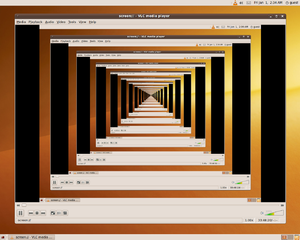
\includegraphics{images/rekursion.png}\end{center}
	\caption{Grafische Rekursion}
\end{figure}

Rekursion bedeutet, dass sich eine Funktion immer wieder selbst aufruft. Um eine sich wiederholende Struktur auszunutzen. Ein einfaches Beispiel dafür ist die Fakultät einer Zahl, wo bereits die Definition rekursiv ist:

\begin{center}
	$1! = 1$
	$n! = n\cdot (n-1)!$
\end{center}

Wie du siehst, wird die Fakultät benutzt um die Fakultät zu definieren. Die Rekursion hat außerdem noch eine Abbruchbedingung, in diesem Fall wenn $n=1$. Wenn ihr eine Rekursion programmiert, müsst ihr auch eine Abbruchbedingung programmieren. Der untenstehende Code ist ein Beispiel für die Fakultät die mit Hilfe von Rekursion gelöst wird.

\begin{minipage}{\textwidth}
\begin{lstlisting}
public class Rekursion{
  public static void main(String[] args){
    long number = 12;
    long result = factorial(number);
    System.out.println(result);
  }
  
  public static long factorial(long number){
    //Abbruchbedingung
    if(number <= 1){
      return 1;
    }
    //rekursiver Aufruf
    return number*factorial(number-1);
  }
}
\end{lstlisting}
\end{minipage}

In der Funktion \textit{factorial} findet ihr beide Elemente, die jede Rekursion enthalten muss. Zum Einen die Abbruchbedingung bei der geprüft wird, ob die Zahl kleiner als 2 ist. Wenn das so ist wird eine Konstante zurückgegeben. Zum Anderen findet ihr den rekursiven Aufruf, bei dem in der \textit{return}-Zeile wieder die Funktion aufgerufen wird.

\section{Aufgaben}

\begin{enumerate}
	\item Du kennst sicherlich den Bereich in diversen Supermärkten in denen die Einkaufswagen stehen. Mit dem Programm ShoppingCart.java wollen wir diesen Bereich jetzt nachbauen.
	\begin{itemize}
		\item Mach aus der Ausgabe eine Funktion mit einem aussagekräftigen Namen.
		\item Schreibe eine Funktion, die einen Einkaufswagen aus einer zufällig gewählten Reihe wegnimmt.
		\item Schreibe eine Funktion, die einen Einkaufswagen in eine zufällge Reihe einfügt.
		\item Schreibe eine Funktion, die den Einkaufswagen in der längsten Reihe wieder einreiht.
		\item Simuliere den Supermarkt in mehreren Schritten. Wenn du es dir leicht machen willst, nimmt der Kunde den Einkaufswagen in einer Phase mit und bringt ihn sofort zurück. Die Fortgeschrittenen Java-Programmierer unter euch können mehrere Kunden im Markt simulieren.
	\end{itemize}
	\item Schreibe ein Programm, dass die n-te Fibonaccizahl ausrechnet.
	\item Schreibe ein Programm, dass die Ackermannfunktion berechnet.
	\item Schreibe ein Programm, das die Fakultät berechnet ohne Rekursion zu benutzen.
\end{enumerate}
